\section{软件测试}

    根据本次毕业设计中的实现内容,软件测试主要分为两大部分,系统功能模块测试及系统整体测试,其中功能模块测试主要包含
    指纹识别模块测试,网卡驱动测试,网络协议栈集成测试几个部分。

    \subsection{指纹识别模块测试}

    本测试主要在上位机中进行,主要目的在于证明可以通过指纹管理程序在不影响指纹识别的情况下
    对于指纹特征数据进行上传和下载(见图\ref{总体设计图})右侧上位机与 FPM383C 之间的连线。

    \subsubsection*{测试准备:}
    硬件层面上需要使用 CH340 TTL转USB模块,杜邦线,指纹识别模块,开发板。
    软件层面上不需要额外准备,直接采用 chainboot 显示对应输出即可。

    经串口发送亮灯信号,对应指纹模块亮灯可见指纹识别模块能与计算机和树莓派建立有效的串口连接。

    \subsubsection{指纹注册测试}
    
    由于按照目前设计,指纹注册功能在上位机中实现。在正确注册指纹之后,通过调用协议使指纹模块上传
    指纹特征信息到上位机,通过 UdpSocket 将对应数据包中信息整合后经过网络分发到下位机
    \footnote{在这段测试中,由于经由网络下发指纹特征信息由于量太多不太容易进行呈现,暂且不进行相关演示}。

    首先通过指纹识别模块配的客户端程序清空上位机从属指纹模块中的指纹模板(如图\ref{fig::清空指纹模板})。

    \begin{figure}[ht]
        \centering
        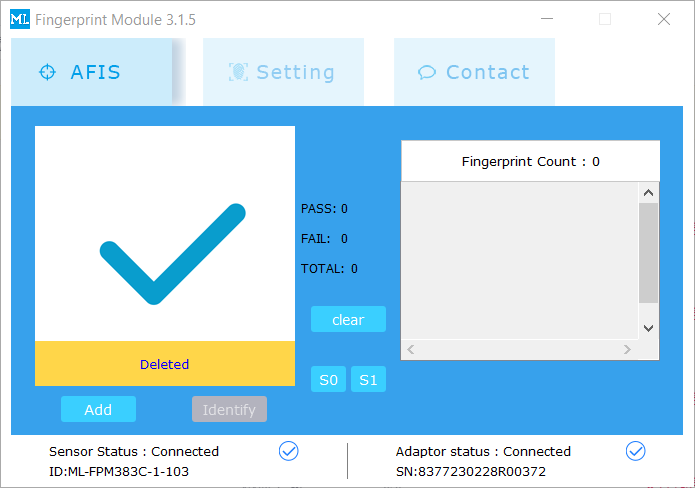
\includegraphics[scale=0.8]{./imgs/清空指纹模板.png}
        \caption{清空指纹模板}    \label{fig::清空指纹模板}
    \end{figure}

    将指纹模块插入到上位机中,通过在上位机中运行的简单注册终端进行注册。
    首先,根据用户信息表(见表\ref{tab:userInfo})中所设计的各项信息进行输入,在输入数据完成校验。
    然后,管理程序调用指纹注册函数,函数在调用指纹模块的自动注册命令完成有关指纹模块的注册后
    自动调用上传指令,
    将对应数据由上位机从属指纹识别模块上传到上位机数据库中 Finger{id}Data 表中
    (见图\ref{test::用户注册} \footnote{图中下半部分输出的字节数据分别代表由串口获取的完整特征信息和其中的指纹信息}),
    并且根据数据库设计,自动完成 users,FingerInfo 等关联表的构建。

    \begin{figure}[ht]
        \centering
        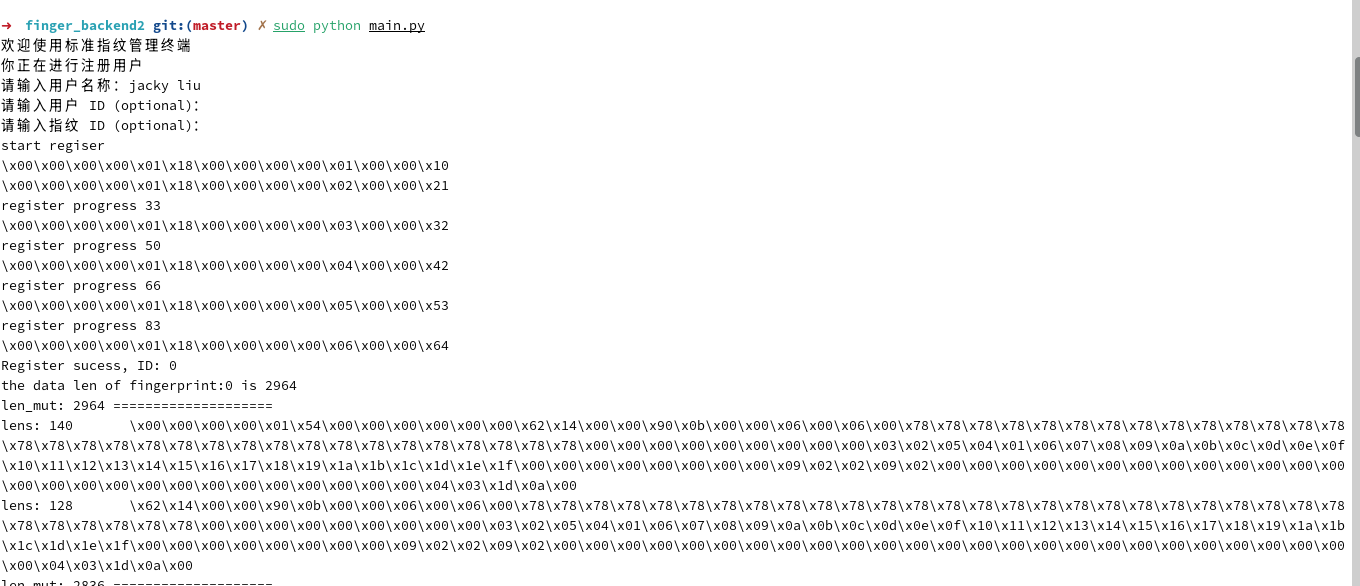
\includegraphics[width=\textwidth]{./imgs/测试-用户注册.png}
        \caption{用户注册}    \label{test::用户注册} 
    \end{figure}   

    完成注册操作之后,由图\ref{test::注册后数据库查询} 可见,对应的表和关系已经正确构建。
    下图中对 FingerInfo 表的查询体现了 finger\_id 0 与 user\_id 1 的映射关系,还保存了指纹特征 0 的长度信息,
    注册的指纹特征信息二进制数据被保存在 Finger0Data 表中。

    \begin{figure}[ht]
        \centering
        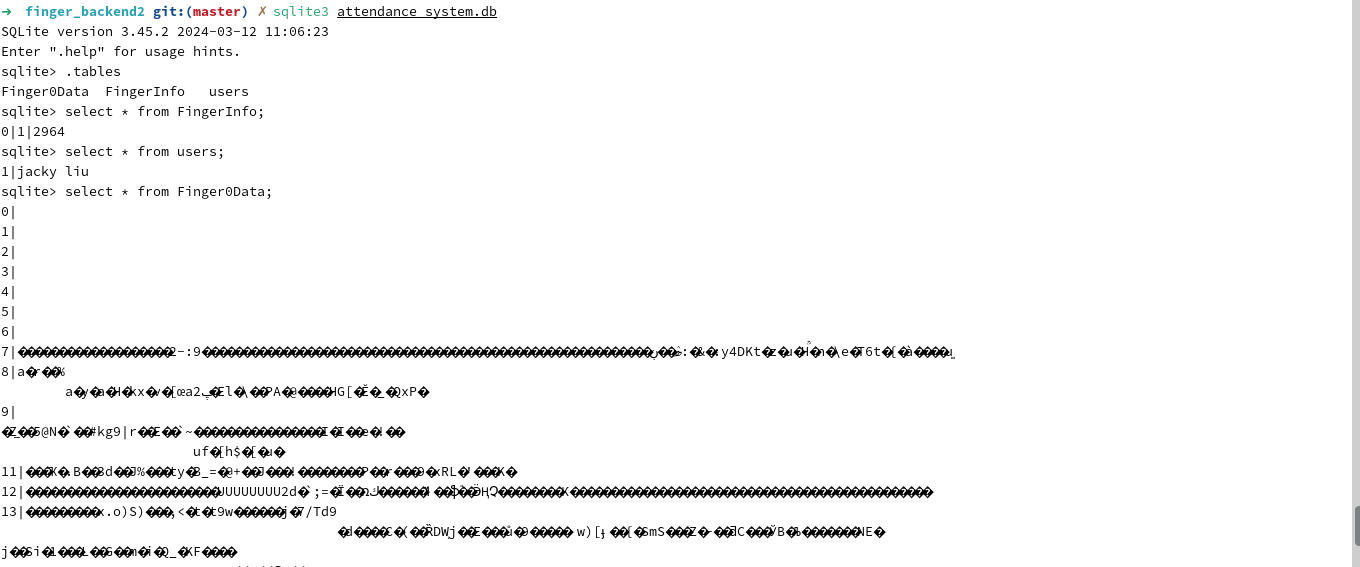
\includegraphics[width=\textwidth]{./imgs/测试-注册后数据库查询.png}
        \caption{用户注册后数据库查询}    \label{test::注册后数据库查询}
    \end{figure}   

    \subsubsection{指纹删除}

    指纹删除功能终端尚未实现,还需要一些时间。

    \subsubsection{指纹下载}

    本测试不属于指纹考勤管理系统的主要组成成分,主要目的在于测试在指纹特征数据的上传和下载中是否出现了信息丢失
    导致指纹无法正常识别的现象。

    首先,先根据指纹注册测试的方式或者是由指纹模块配的指纹管理程序完成指纹注册(见图\ref{fig::注册指纹})后单独进行指纹上传操作。
    然后,由指纹模块配的指纹管理程序删除注册的指纹(见图\ref{fig::清空指纹模板})
    \footnote{删除测试的方法会一并删除指纹特征文件与关联图等内容}。

    \begin{figure}[ht]
        \centering
        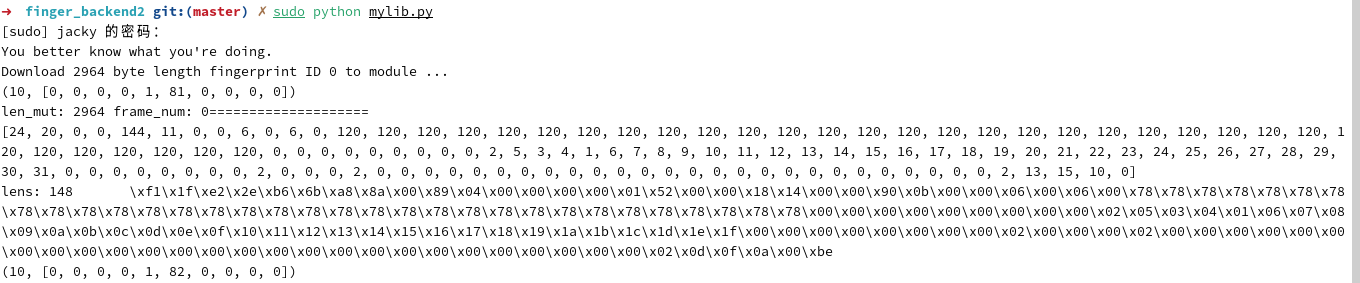
\includegraphics[width=\textwidth]{./imgs/测试-指纹上传.png}
        \caption{指纹上传}    \label{test::指纹上传}
    \end{figure}   

    \noindent
    \begin{minipage}[t]{0.48\linewidth}
        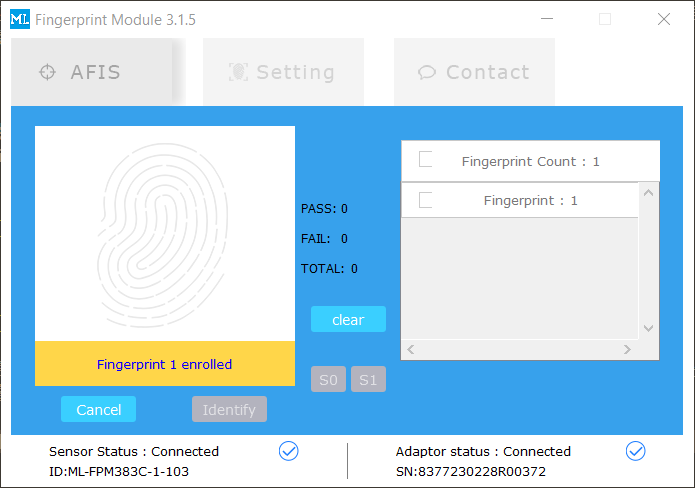
\includegraphics[width=\textwidth]{./imgs/注册指纹.png}
        \captionof{figure}{指纹客户端注册指纹}    \label{fig::注册指纹}
    \end{minipage}
    % \quad
    \begin{minipage}[t]{0.48\linewidth}
        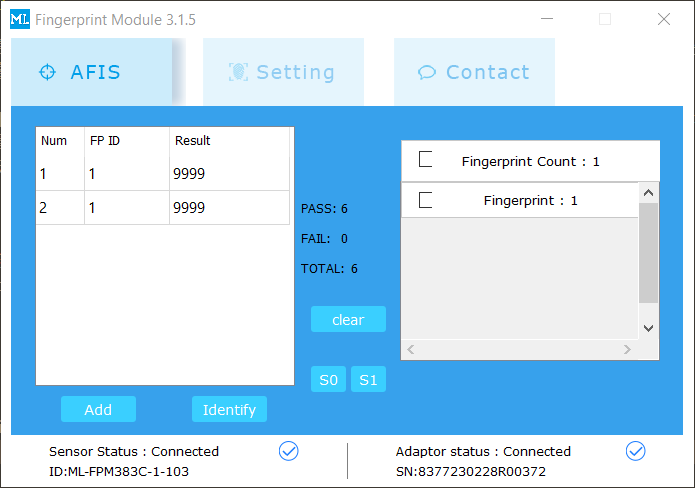
\includegraphics[width=\textwidth]{./imgs/测试-指纹上传后查询与匹配.png}
        \captionof{figure}{指纹上传后查询与匹配}    \label{test::指纹上传后查询与匹配}
    \end{minipage}

    如图 \ref{test::指纹上传} 可见通过执行内置指纹上传函数实现的指纹上传输出,
    其中 (10, [ ..., 0, 81, ... ]) 代表执行 upload 指令时的回返信息,
    第一段数组代表由数据库中读取的二进制指纹特征信息(一帧),
    第二段字节代表整个由上位机经由串口下发到指纹识别模块的串口信息。

    将指纹识别模块重新接入上位机中(如图\ref{test::指纹上传后查询与匹配})可见,
    之前删除的左手大拇指指纹已经重新被识别出来了,并且经过两次指纹匹配测试均能保证
    识别准确率能够达到 100,这无疑证明了在指纹特征信息由指纹模块中上传再下载的过程中
    并没有对于指纹特征信息的完整性进行破坏,上传再下载的行为也不会导致指纹特征信息被破坏。

    \subsection{以太网卡驱动测试}

    本测试主要目的在于通过测试实现的以太网驱动是否能够实现以太网帧的收发,
    以及发送带宽说明以太网驱动实现的效果。

    本章节的主要呈现流程如下:首先,先通过两台通用 PC 机对于测试与接收程序的效果进行分析,
    然后将对应接收脚本转移到 树莓派 Linux 环境下进行本地编译收发包测试,
    虽然固然存在 C,Rust 所导致的差异,但是由于 C 语言标准库尚未提供对于以太网帧的直接收发功能
    因此没有办法在以太网帧层面进行 Rust 下的对比。

    \subsubsection{测试脚本测试}

    按照一开始的测试计划,应该采用两台电脑进行测试,一台电脑通过 WSL(windows subsystem of linux) 
    运行 linux 测试发包脚本,另外一台笔记本通过 RJ45转USB模块\footnote{或者说叫做usb网卡}
    经由双绞线与前者进行连接。

    但是按照这种操作流程进行测试的时候,实际上并没有办法实现以太网帧的收发,
    经过分析之后发现产生这种问题的主要原因的是 WSL 与 宿主机 之间的网络连接方式是通过
    类似于 NAT 的方式进行连接的,在这种情况下,WSL 与 宿主机之间存在一个子网,因此
    在 WSL 中在以太网帧层面实现的收发只能在,并不能在宿主机上获得转发,因此
    另外一台 linux PC 没有办法收到对应以太网帧。
    \footnote{IP层以上的包会自动被转发,但以太网帧不会}

    最终,采用了两台运行 linux 操作系统的电脑进行此测试(其中一台采用 nixos live,一台是 nixos)。
    \footnote{由于其中一台仍通过 RJ45转USB模块 实现网络收发功能同时配有百兆网卡,因此本次测试中的最高传输速率仅为100mbps}
    二者均在完全关闭防火墙,配置对应以太网卡的 ip 地址,并实现相互 ping 之后展开测试。
    发包侧(如附录代码段 \ref{code::eth-send})在十秒内持续发送以太网帧,并且在以太网帧的第 16 位开始的八个字节添加代表当前以太网帧序号的八个字节 (unsigned long long)数据。
    收包侧(如附录代码段 \ref{code::eth-recv})按照对应收包顺序与检测出的序号综合进行判断在传输过程中是否存在丢包,乱序的情况。

    其中初步测试情况说明可能存在三种情况:

    \begin{enumerate}
        \item 收发端收发包数量一致当前测试完整完成。
        \item 收发端数量不一致可能说明在收发的过程中存在由于溢出或其他原因导致的丢包情况
        \item 收发端数量一致,但是存在丢包,可能说明 C 程序调用裸套接字实现以太网帧的发送过程中,
        会自动调用对应的重发功能,从某种程度上可以证明传输的质量。
    \end{enumerate}

    具体测试结果见下\ref{tests::测试脚本测试}表,在以太网帧百兆层面不存在丢包的情况,
    并且可以较好的实现前面所需求的测试结果。

    \begin{table}[ht]
    \centering
    \label{tests::测试脚本测试}
    \caption{测试脚本测试表}
    \csvautobooktabular{./imgs/测试记录-测试脚本测试.csv}
    \end{table}

    \subsubsection{树莓派网络传输速率测试}

    本测试主要想要实现的效果在于测试出在树莓派直接采用 Linux 镜像原装的网卡驱动所能实现的传输效率,以方便与后面
    我们通过 Rust 在 ArceOS 裸机上实现的网卡驱动(以太网帧)测试出的收发效率进行对比。

    具体操作流程基本上与前章节保持一致,除了其中一台百兆网卡的测试PC被更换成为了树莓派,
    二者直接通过双绞线进行连接。
    
    其中测试出以太网帧与传输速率直接的关系如下图 \ref{tests::Linux网卡驱动传输率与以太网帧大小} 所见,测试记录见附录表 2-1。
    根据图所知,以太网帧大小与树莓派传输速率之间存在指数关系,
    并且以太网帧越大,在同等时间内的以太网传输速率越大,在以太网帧层面网络传输速率最大能达到983.mbps,
    接近树莓派千兆网卡的理论最大传输速率。

    \begin{tikzpicture}
        \centering
        \begin{axis}[
            xlabel={以太网帧大小}, ylabel={传输速率},
            xmin=0,
            width=0.8\textwidth,
            legend pos=south east,
            grid=both
        ]
        
        \addplot[thick, mark=*, blue] coordinates {
            (64, 112.3833333)
            (128, 233.0333333)
            (256, 456.5257143)
            (512, 739.01)
            (1024, 898.616)
            (1280, 943.565)
            (1408, 949.85)
            (1500, 946.8366667)
        };
        \addlegendentry{发送速率}
        
        \addplot[thick, mark=*, red] coordinates {
            (64, 112.3833333)
            (128, 233.0333333)
            (256, 445.5085714)
            (512, 734.5766667)
            (1024, 889.338)
            (1280, 938.1825)
            (1408, 949.85)
            (1500, 938.5266667)
        };
        \addlegendentry{接受速率}

        \end{axis}
    \end{tikzpicture}
    \captionof{figure}{树莓派Linux驱动传输率与以太网帧大小}    \label{test::Linux网卡驱动传输率与以太网帧大小}

    \subsection{网卡驱动测试}

    本测试主要目的在于测试在 ArceOS 下的以太网卡驱动传输速率,并且最终与树莓派网络传输速率进行对比,评价以太网网卡驱动的实现效果。
    由于后面在将以太网卡驱动与 ArceOS 网络协议栈进行嵌合的时候对于以太网卡驱动进行了破坏性修改
    \footnote{BCM54213PE驱动中调用ArceOS函数是通过PhantomData间接调用traits实现来完成的}。
    因此,本次测试由完成了网络驱动测试的 \href{https://bitbucket.org/jackyliu16/arceos/commits/92e9b6abcdf180359381088552688c0fcbc83bf2}{commit} 
    分叉出 \href{https://bitbucket.org/jackyliu16/arceos/commits/branch/ethernet-test}{ethernet-test}
    分支,并在此分支中完成了对应测试。

    \subsubsection{发包测试}

    由树莓派向上位机直接发送以太网帧,在上位机中通过 wireshark 进行抓包(如图\ref{test::以太网通信正常})

    \begin{figure}[ht]
        \centering
        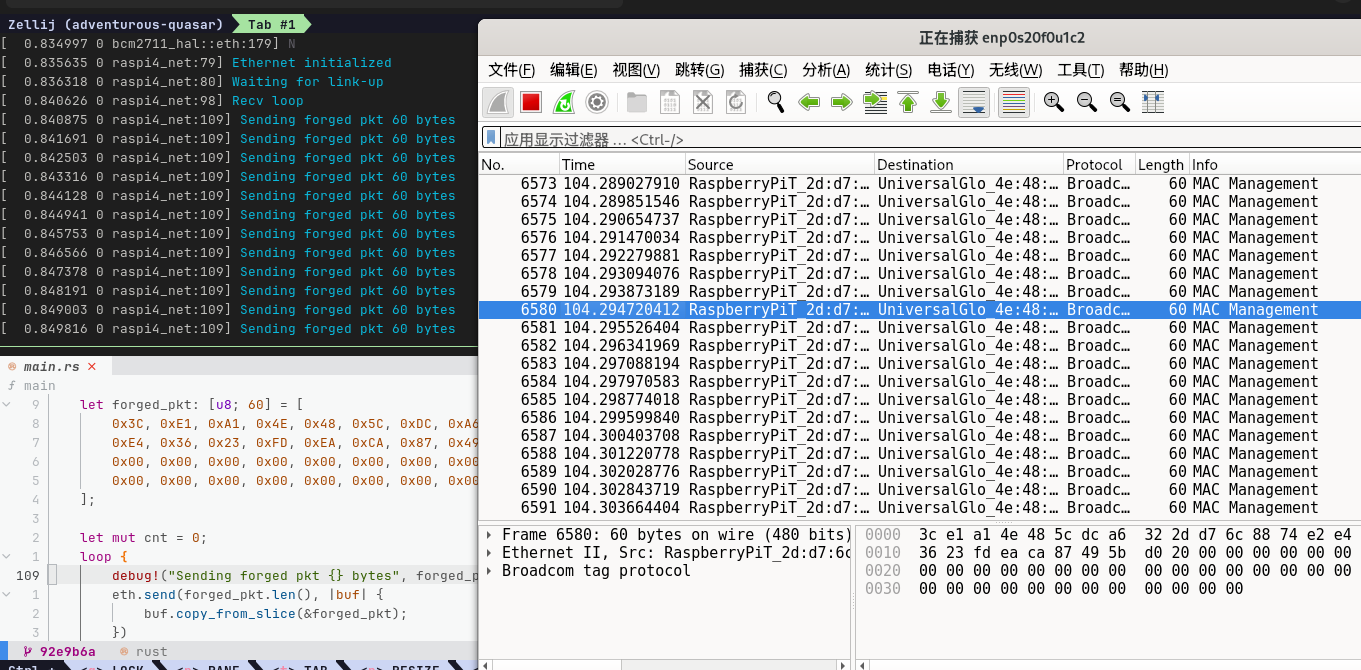
\includegraphics[width=\textwidth]{./imgs/以太网帧通信正常.jpg}
        \caption{以太网帧通信正常}    \label{test::以太网帧发送}
    \end{figure}   

    \subsubsection{收包测试}

    在树莓派上直接收包并打印对应信息(见图\ref{test::以太网帧接收})。
    由于目前树莓派并没有实现网络协议栈,因此
    无法通过如 nc, nping 等基于网络的传输工具向树莓派发送自定义以太网帧。
    因此,此处直接使用了 nc 随便发送了一段数据到树莓派中。
    此处指定的网段与上,下位机网段一致,因此会在上位机的特定端口中释放 ARP 探寻包,
    如图所示,对应的 ARP 探寻包被正确解析,因此可以浅薄的认为以太网驱动收包正常。

    \begin{figure}[ht]
        \centering
        \begin{subfigure}
            \centering
            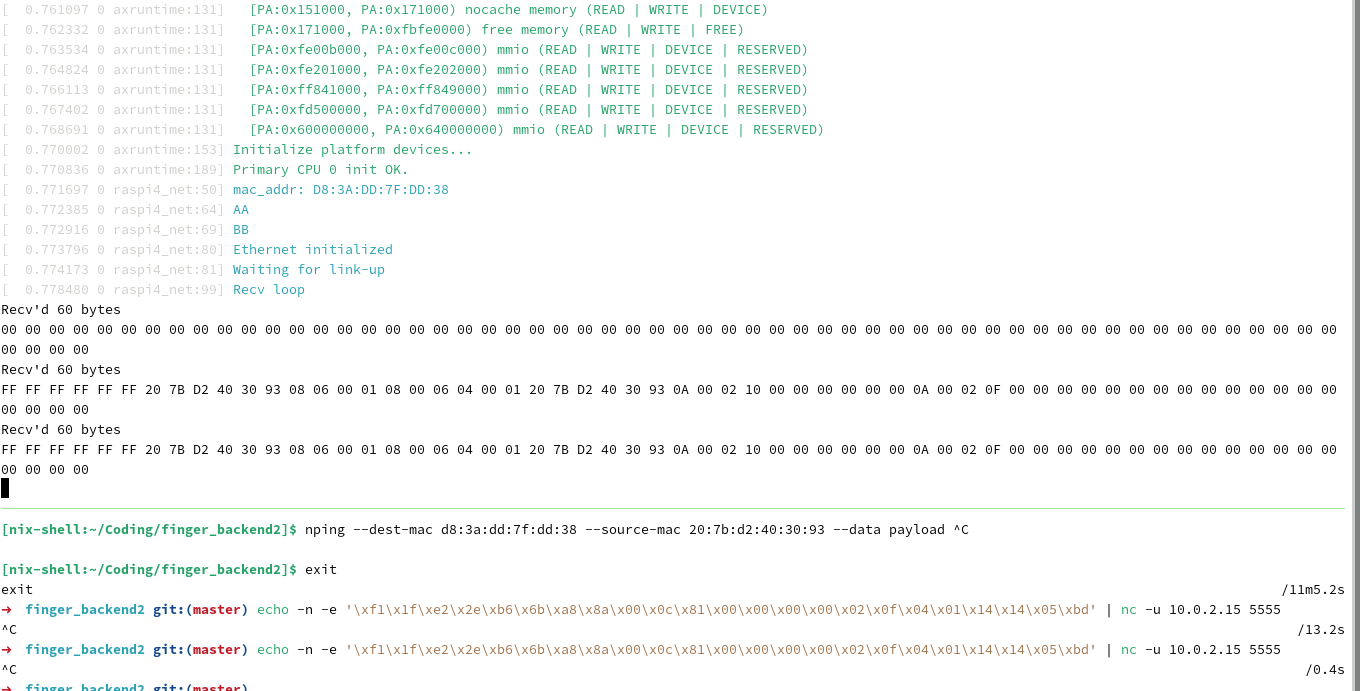
\includegraphics[width=\textwidth]{./imgs/测试-以太网帧接收.png}
        \end{subfigure}
        \hfill
        \begin{subfigure}
            \centering
            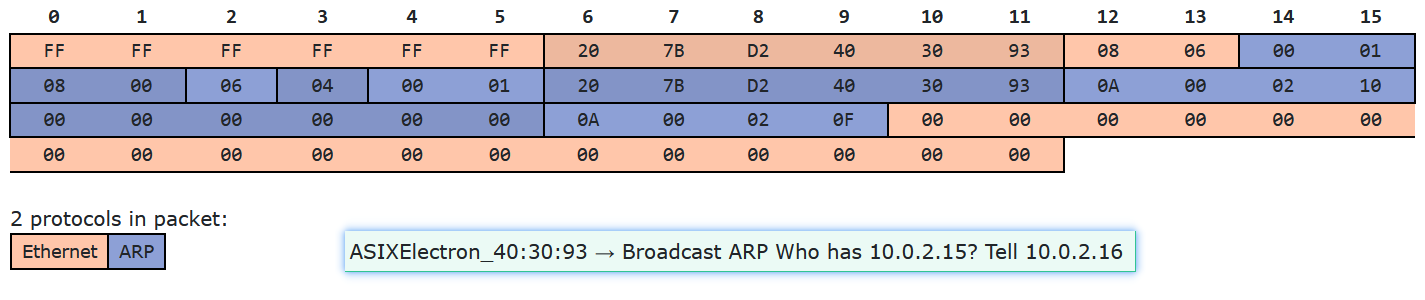
\includegraphics[width=\textwidth]{./imgs/测试-以太网帧接收-解析.png}
        \end{subfigure}
        \caption{接受的以太网帧及解析} \label{test::以太网帧接收}
    \end{figure}

    \subsubsection{传输速率测试}

    \begin{tikzpicture}
        \centering
        \begin{axis}[
            xlabel={以太网帧大小}, ylabel={传输速率},
            xmin=0,
            width=0.8\textwidth,
            legend pos=south east,
            grid=both
        ]
        
        \addplot[thick, mark=*, blue] coordinates {
            (60, 195.29)
            (128, 409.73)
            (256, 695.9225)
            (384, 941.24)
            (512, 955.32)
            (768, 969.84)
            (1024, 977.3)
            (1280, 981.84)
            (1408, 983.52)
            (1500, 984.55)
        };
        \addlegendentry{发送速率}
        
        \addplot[thick, mark=*, red] coordinates {
            (60, 189.773072)
            (128, 365.4372917)
            (256, 685.4498305)
            (384, 937.4238723)
            (512, 950.7467263)
            (768, 966.6822143)
            (1024, 973.7869313)
            (1280, 974.960128)
            (1408, 975.087309)
            (1500, 979.688400)
        };
        \addlegendentry{接受速率}

        \end{axis}
    \end{tikzpicture}
    \captionof{figure}{树莓派Linux驱动传输率与以太网帧大小}    \label{test::Linux网卡驱动传输率与以太网帧大小}


        \begin{tikzpicture}
        \centering
        \begin{axis}[
            xlabel={以太网帧大小}, ylabel={传输速率},
            xmin=0,
            width=0.8\textwidth,
            legend pos=south east,
            grid=both
        ]
        
        \addplot[name path=linux, thick, mark=*, orange] coordinates {
            (64, 112.3833333)
            (128, 233.0333333)
            (256, 445.5085714)
            (512, 734.5766667)
            (1024, 889.338)
            (1280, 938.1825)
            (1408, 949.85)
            (1500, 938.5266667)
        };
        \addlegendentry{Linux 驱动}
        
        \addplot[name path=arceos, thick, mark=*, blue] coordinates {
            (60, 189.773072)
            (128, 365.4372917)
            (256, 685.4498305)
            (384, 937.4238723)
            (512, 950.7467263)
            (768, 966.6822143)
            (1024, 973.7869313)
            (1280, 974.960128)
            (1408, 975.087309)
            (1500, 979.688400)
        };
        \addlegendentry{ArceOS 驱动}

        \addplot fill between[
            of = linux and arceos,
            soft clip={domain=0:1500},
            every even segment/.style  = {gray,opacity=.4}
        ];

        \end{axis}
    \end{tikzpicture}

    基于前面的测试,说明当前以太网帧的收发功能是正常的,此处使用一个简单的发送 buf
    的循环尝试对于以太网驱动的传输速率进行测试。

    从目前来看,在此次测试中有且存在两个变量, 一个是以太网帧的长度,另一个是每次发送之间的间隔。
    在十秒钟内测试以太网驱动的最大每秒兆比特,并且根据其与 BCM54213PE PHY 芯片的
    理论最高每秒兆比特进行对比,来说明以太网驱动的实现效果。

    其中采用以太网帧大小作为其中的一个参数的主要原因在于需要对以太网驱动在帧间的消耗时间
    进行评估,而发送时间间隔则是为了解决由于以太网帧在短时间内急剧增加,新增速率低于
    消耗速率导致的溢出问题\footnote{在本驱动中尚没有考虑到这个问题的解决}。
    具体测试记录见附表(TODO:将最终测试表插入到附录)。

    $$\text{mbps} = \frac{\text{total\_bytes} \times 8.0}{\text{elapsed\_secs} \times 1,000,000.0}$$

    根据测试记录(见附录分析,其中以太网帧大小与以太网帧传输速率之间存在对数关系(如图\ref{test::传输率与以太网帧大小}所示)
    对数关系在以太网帧长度为 375 字节时达到最高点 94.3 MBps,与 BCM54213PE 千兆网卡的理论最大
    传输速率 125MBps 相差不大。但在长度超过 375 字节之后,以太网帧长度再继续增加会产生未定义行为,
    该行为具体表现为上位机 wireshark 只能按照规定长度抓到头几个包,后面的包没有被发送到网络中。
    同时,计算得出的每秒兆比特也远远超过了 BCM54213PE 的理论最大传输率,
    如以 512 字节的以太网帧,间隔 10500 纳秒以下,
    计算结果为 149.21MBps,远远超过了千兆网卡的理论最大传输率 125MBps。

    \begin{tikzpicture}
        \centering
        \begin{axis}[
            xlabel={以太网帧大小}, ylabel={传输速率},
            xmin=0,
            width=0.8\textwidth,
            legend pos=north east,
            grid=both
        ]
        
        \addplot[only marks
        , mark=*
        , blue
        ] table [x=EthPackSize, y=AvgBandwidth, col sep=comma] {./imgs/测试记录-传输率与以太网帧.csv};
        \addlegendentry{测试数据}
        
        % 添加趋势线 A + B * Exp(c * X)
        \addplot[thick, green, domain=64:1000] {94.66701212555364 - 43.26235037169133 * exp(-0.010715300001686431 * x)};
        \addlegendentry{指数趋势线}

        % \addplot[dashed, black, thick] coordinates {(64, -10) (64, 100)}; % 调整 y 范围以适应图表
        % \node at (axis cs:64, 100) [anchor=north] {64};
        
        \end{axis}
    \end{tikzpicture}
    \captionof{figure}{传输率与以太网帧大小}    \label{test::传输率与以太网帧大小}

    % \begin{figure}[ht]
    %     \centering
    %     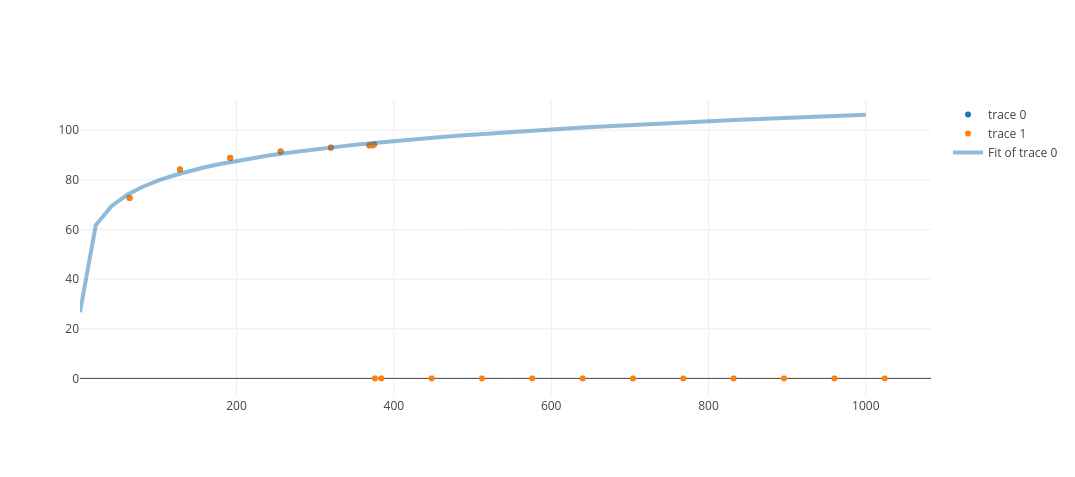
\includegraphics[width=\textwidth]{./imgs/测试-传输率与以太网帧大小.png}
    %     \caption{传输率与以太网帧大小}    \label{test::传输率与以太网帧大小}
    % \end{figure}   

    根据这样的测试结果,我提出了一个简单的设想,即产生这种现象的原因在于以太网驱动没能及时
    将收到的包传输出去,导致后面的包实际上并没有执行发送行为,而是在资源复用的时候被阻挡自动返回了。
    因此,引入了传输延迟作为参数的一部分以方便对于最大传输率进行测试。

    该参数虽然会导致同等情况下传输速率下降(如图\ref{test::传输率与发送延迟}所示)
    ,但是他的引入可以使原先无法正常发送的以太网帧长度正常发送,如 376 字节的以太网帧在没有引入
    传输延迟的时候是没有办法正常完成发送的,但是引入不到 150 纳秒的延时就可以使之正常运行,同时还提升了传输速率到 94 MBps,从某种程度上
    来说可以提升网络传输效率。

    \begin{tikzpicture}
        \centering
        \begin{axis}[
            xlabel={发送延迟}, ylabel={传输速率},
            xmin=0,ymax=100,
            width=0.8\textwidth,
            legend pos=north east,
            grid=both
        ]
        
        \addplot[only marks
        , mark=*
        , blue
        ] table [x=Delay, y=Bandwidth with 128 EthPackSize, col sep=comma] {./imgs/测试记录-传输率与传输延迟.csv};
        \addlegendentry{测试数据}
        
        % 添加趋势线 A + B * Exp(c * X)
        % \addplot[thick, green, domain=0:1000000] {660066.98 * x^-0.96};
        \addplot[thick, green, domain=10000:1000000] {839028.750214695 * x^-0.983848891456114};
        % \addplot[thick, green, domain=0:1000000] {7.2132943561133525 + 130.53328368716328 * exp(-0.000052669151121911975 * x)};
        \addlegendentry{指数趋势线}

        \end{axis}
    \end{tikzpicture}
    \captionof{figure}{传输率与发送延迟}    \label{test::传输率与发送延迟}

    \subsection{网卡协议栈集成测试}

    通过双绞线将树莓派的 RJ45 网口与笔记本端口相连,在笔记本上运行 server.py 程序(打开 5555 端口)
    清空所有防火墙设置,并且设置端口 5555 的出入站规则,将笔记本以太网网卡 ip 地址设置为
    树莓派默认 ip 地址 10.0.2.15 同一网段下的 10.0.2.16\footnote{见指纹识别模块flakes初始化语句}。

    \subsubsection{Udp 发包测试}

    在应用程序中,使用 axstd 替代 rust std 库,创建 UdpSocket,调用 sendto 方法,
    向上位机的 5555 端口发送测试连接字节数组(如图\ref{test::Udp发包}所示)。

    \begin{figure}[ht]
        \centering
        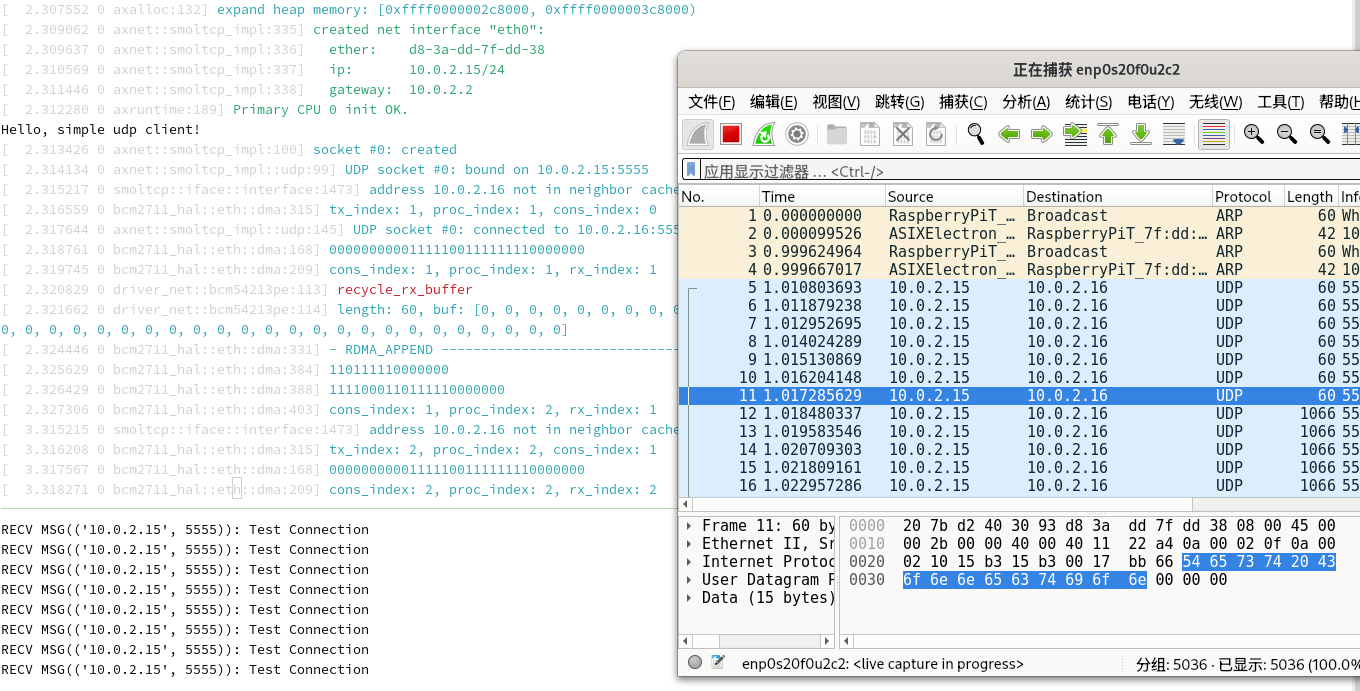
\includegraphics[width=\textwidth]{./imgs/测试-udp发包正常.png}
        \caption{Udp发包正常}    \label{test::Udp发包}
    \end{figure}   

    \subsubsection{Udp 收包测试}

    UdpSocket 收包测试我主要根据两种常见的网络联通方式进行测试,即 Netcat 和 ping。
    首先,针对 ARP,ICMP 包的测试(如图\ref{test::pingICMP回返测试}所示)。
    其中左上角是串口面板,右上角是正在运行中的 server.py 程序,左下角是
    执行的指令,即 ping 10.0.2.15。
    
    根据 ping 的一般操作流程,首先上位机中会先通过 ARP 探寻包,询问 10.0.2.15
    IP 地址所对应的硬件 MAC 地址,在下位机回返 MAC 地址后,连接被建立。
    上位机发送 ICMP Echo 请求到下位机,下位机以太网协议栈对收到的 ICMP 包进行处理,
    发送 ICMP Echo 作为回复。

    \begin{figure}[ht]
        \centering
        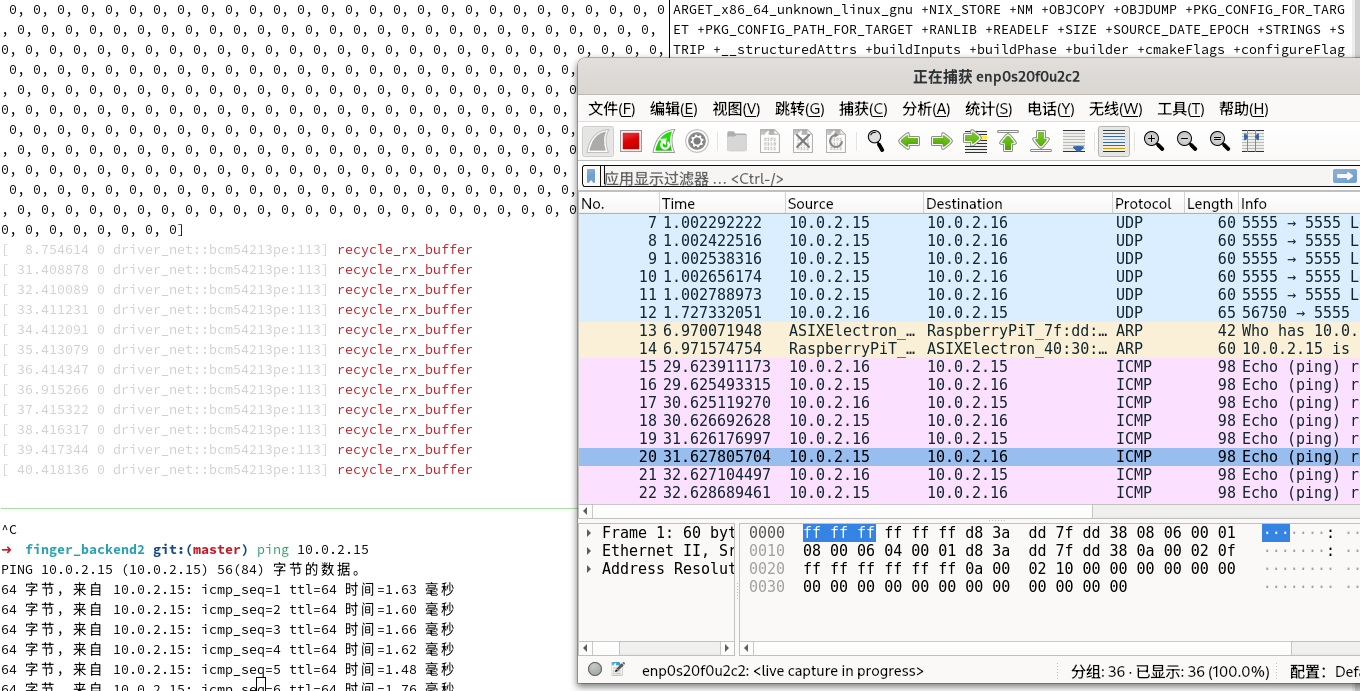
\includegraphics[width=\textwidth]{./imgs/测试-pingICMP回返测试.png}
        \caption{ping 回返测试}    \label{test::pingICMP回返测试}
    \end{figure}   

    然后,根据指纹考勤系统由上位机经由网络向下位机发送指纹信息的需求,
    我对于 Udp 连接进行了简单的测试。即通过 netcat 直接将一个字节数组
    (指纹模块的 LED 控制信号)
    由上位机传输到下位机,由图\ref{test::接收netcat数据}所示,下位机中
    缓冲区的字节数据与上位机中通过 netcat 传输的字节数据完全一致
    \footnote{这个地方没有对边界进行判断,直接打印了整个缓冲区}。

    \begin{figure}[H]
        \centering
        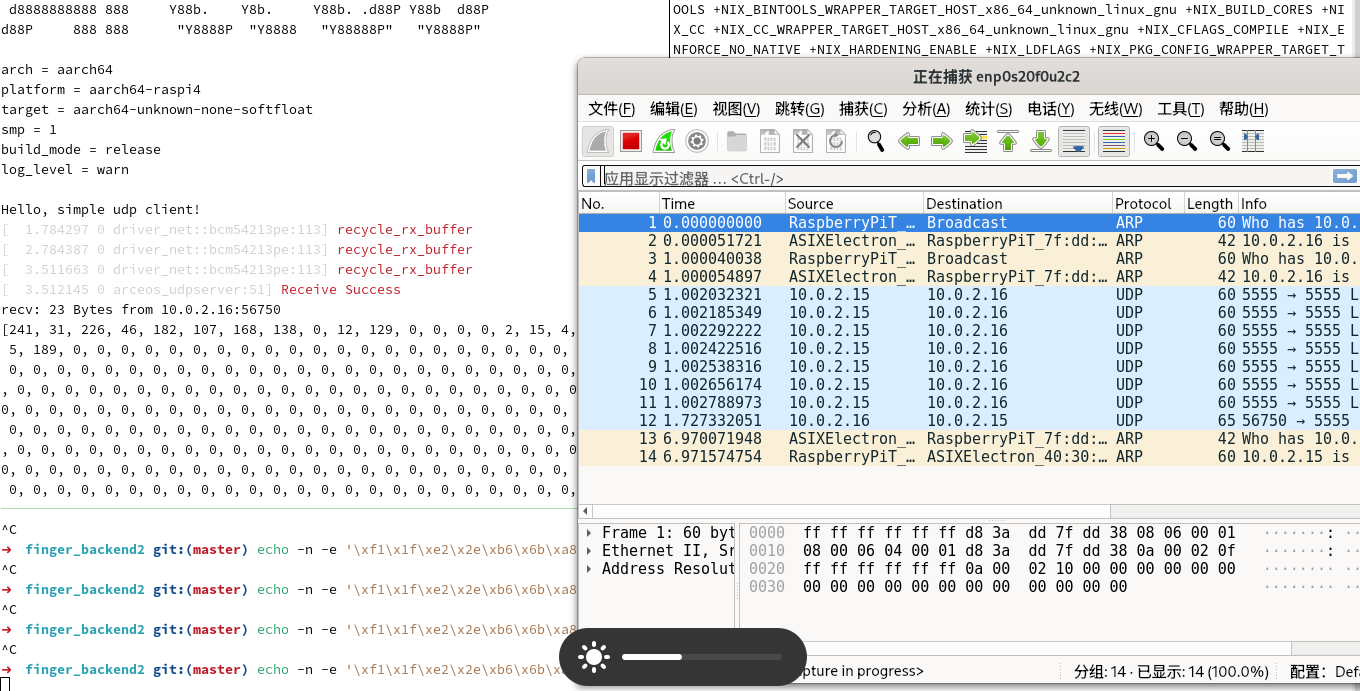
\includegraphics[width=\textwidth]{./imgs/测试-接收netcat数据.png}
        \caption{接收netcat数据}    \label{test::接收netcat数据}
    \end{figure}   

    \subsubsection{传输速率测试}

    尚未完成,目前仅测试 120\_000 纳秒传输延时情况下传输速率
    最大能达到 53.64 MBps。

    \subsection{集成测试}

    尚未完成

    \subsubsection{指纹打卡及信息上传}

    尚未完成

    \subsubsection{指纹同步}

    尚未完成